
\section{notes thesis}

put fig. somewhere earlier (p.~10?): see \autoref{fig:Hundhausen1977_fig20bcd}\\
\begin{figure}[htb]
	\centering
	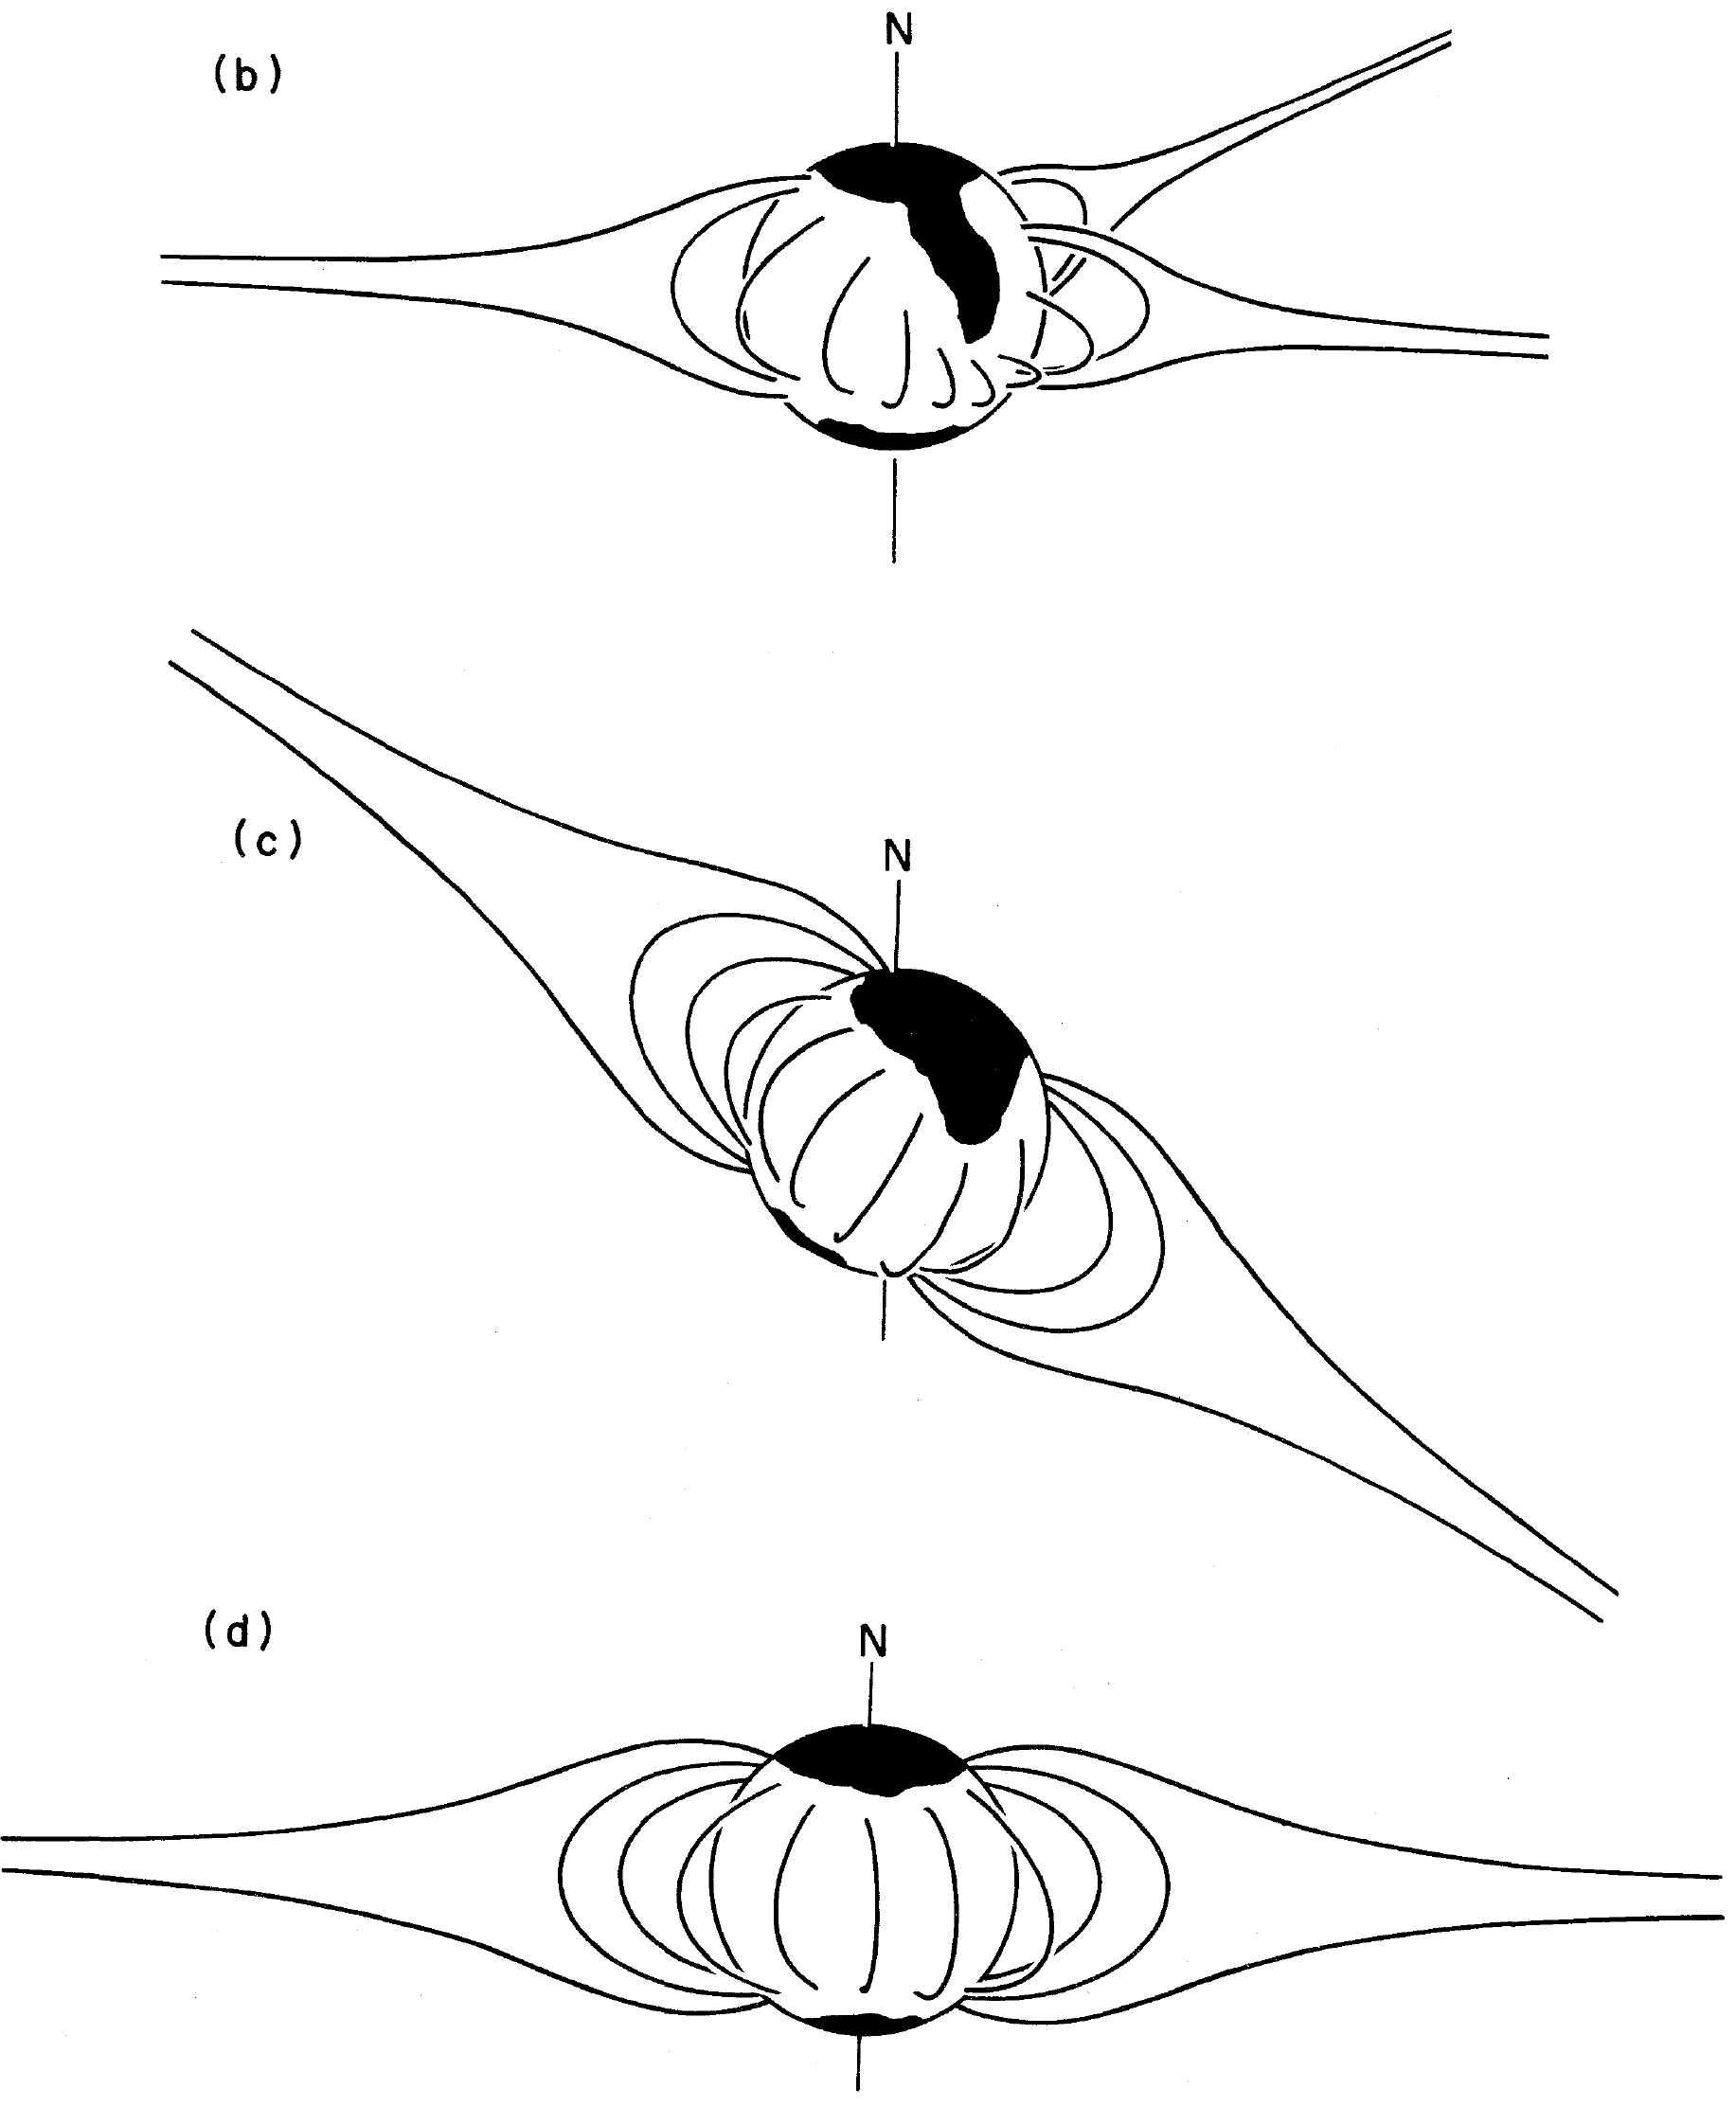
\includegraphics[width=0.5\textwidth]{figures_of_others/images/Hundhausen1977_fig20bcd.png}
	\caption[\lofimage{figures_of_others/images/Hundhausen1977_fig20bcd.png}Credit: {\citep[Fig.~20, panels (b--d)]{Hundhausen1977}}, \textcopyright~Colorado Associated University Press, reproduced with permission.]
	{Schemata of different coronal configurations during the solar cycle. Visualized are the locations of closed coronal magnetic fields (lines) and coronal holes (black areas) for a post maximum distorted dipole (top panel), for a pre minimum stable tilted dipole (middle panel), and a post minimum axial dipole (bottom panel). Credit: {\citep[Fig.~20, panels (b--d)]{Hundhausen1977}}, \textcopyright~Colorado Associated University Press, reproduced with permission.}
	\label{fig:Hundhausen1977_fig20bcd}
\end{figure}

causes (see citet{Rangarajan1997} p.~1282 and mention Bartels1963 too)\\

\citet{Sonnerup1967}: The rotational discontinuity seems to occur predominantly during magnetic storms and two of these cases, involving substantial normal-field components, provide compelling evidence that field reconnection takes place during the storm main phase.\\

% mass flux considerations:\\
% mass per second per Earth disc...\\
% R_E = 6371.008 km\\
% A_E = pi * R_E² = 127 516 438.219 km²\\
% m_p = 1.672621898e-27 kg\\
% v = 400 km/s\\
% n = 6.5 cm-3 = 6.5e15 km-3\\
% mass flux_E = m_p * n * v * A_E = 0,554538384917 kg/s\\
% = 555 g/s = 1996 kg/h = 48 t/d = 17487 t/a\\
% mass per second per magnetosphere disc...\\
% R_MP = 15 * R_E
% A_MP = pi * R_MP² = 28 691 198 599.3 km²\\
% mass flux_MP = 124,772770348 kg/s\\
% = 449 t/h = 10 780 t/d = 3 934 834 t/a\\

% Wikipedia: https://en.wikipedia.org/wiki/Solar_wind
% The wind exerts a pressure at 1 AU typically in the range of 1–6 nPa (1–6×10−9 N/m2), although it can readily vary outside that range.
% The ram pressure is a function of wind speed and density. The formula is
% P = mp * n * V2= 1.6726×10−6 * n * V2
% where mp is the proton mass, pressure P is in nPa (nanopascals), n is the density in particles/cm3 and V is the speed in km/s of the solar wind.[citation needed]

% HCS
why HCS? what currents are there...\\
why is the CS not the divide between both polarities?\\

% space weather
"The principal users affected by geomagnetic storms are the electric power grid, spacecraft operations, users of radio signals that reflect off of or pass through the ionosphere, and observers of the aurora." NOAA cite\\

strong radio bursts; are they relevant direct disturbances for space weather?\\

The solar wind total energy flux at Earth ($1.45~\text{mW/m}^2$) is only about one millionth of the solar radiation flux at Earth (see \citet[p.~153]{Schwenn1990}).\\

% magnetosphere
Phan2005, Magnetopause Processes:\\
Cluster findings include:\\
A strong ‘guide field’ detected at a reconnection X-line, i.e., a finite magnetic field along the X-line, has provided direct evidence for component merging.\\
Tailward-of-the-cusp reconnection has been found to occur only when the IMF has a northward component. The occurrence rate of cusp reconnection is nearly 100\% when the IMF has a northward component, implying that cusp reconnection in the northern and southern hemispheres must be common. The high occurrence rate (in contrast to a rate of 50\% at the subsolar magnetopause) is thought to be due to the presence of a plasma depletion layer. In this layer, the plasma beta is reduced, rendering the magnetosheath flow sub-Alfvenic and allowing the establishment of a stable X-line at the high-latitude magnetopause.\\

look into printed paper collection...\\

% geomagnetic indices
\citet{Lockwood2014} even used geomagnetic indices (including $aa$) to reconstruct the near-Earth IMF strength and solar wind flow speed back to 1845.\\

% halo CMEs:
observed coronal transient: 3d structure, directed at Earth, associated with shock wave; \citep{Howard1982} -> halo CME\\

% chapter2
This work adopts these assumptions and treats the solar wind throughout as a proton plasma.\\

% Kp forecast models
% Aleksei's f/c model; Ukraine; developed within AFFECTS project Space Research Institute of NAS of Ukraine and SSA of Ukraine, Ukraine (SRI NASU-NSAU)\\
% http://www.ikd.kiev.ua/index.php?option=com_content&view=article&id=22%3A2011-02-09-12-19-54&catid=12&Itemid=15&lang=en

% The $\text{d}\Phi / \text{d}t$ coupling relation is being implemented into CME forecast procedures \citep{Savani2017}.\\
% NASA's Space Weather Research Center (SWRC); the derived Kp estimates using real-time in-situ data from L1 are currently implemented within the CCMC integrated Space Weather Analysis System (iSWA); Community Coordinated Modeling Center (CCMC) at the Goddard Space Flight Center\\

% coupling functions
\citet{Elliott2013}: The \Kp~index and solar wind speed relationship: Insights for improving space weather forecasts\\

% Kp index
There exist several indicators/quantities that scale or are based on the \Kp{}~index:
\begin{itemize*}
	\item The equatorward auroral boundary position correlates with the \Kp~index (cite?).
	\item The variation of the total electron content (TEC) of the ionosphere correlates with the \Kp~index (cite?). The TEC has influence on global navigation satellite systems (GNSS). A part of their positional error scales directly with TEC (in extreme cases up to about \SI{30}{\m}).
\end{itemize*}

% solar wind impacts
These solar wind real-time data are used to nowcast various effects on the Earth's magnetosphere, such as the position of the magnetospheric bow shock in front of the Earth, the magnitude of geomagnetic disturbances, the positions of the polar auroral ovals, the variation of the total electron content (TEC) of the ionosphere, and the positional error of global navigation satellite systems (GNSS).\\

% % % chapter2 notes
Savani2017:\\
The Kp difference of 1.5 is tested as there is evidence that a limitation in accuracy is present in the underlying empirical Kp formulation [Mays et al., 2015a]. [...] which is approximately consistent with recent results by Mays et al. [2015a], the Kp empirical formulation is accurate to about Kp = 1.5.\\

What kind of solar wind structures create the individual regions in this distribution? (B--v--\Kp{} circle plot)\\
What is their individual contribution to the \Kp{} ranges (e.g. high \Kp{}: CMEs 70\% and CIRs 30\%)?\\

How can the impact field strength of CMEs be forecasted (v->B correlation for CMEs)?\\
Internal solar wind correlations: B--v correlation\\
ACE MAGSWE 64~s data -> yearly overlay plot\\

Using \vBz{} implies that both quantities are sufficiently independent. $B$ and $v$ are dependent, as can be seen from fig~XX, however, as $v$ and $\theta_c$ are, so are $v$ and $B_\text{z}$, see fig~XX.\\

rt data errors/gaps... vs science data (see paper Kp as V replacement: \citet{Machol2013})\\
DSCOVR as replacement was launched on 11~Februar 2015. It is NOAA's SWPC real-time solar wind prime source since 27 July 2016.\footnote{\urlfoot{http://www.swpc.noaa.gov/products/real-time-solar wind}}\\


% % % chapterPSP notes

% proton flux conservation
larger errors should be located near CMEs and CIRs (nonradial flows from deflections)\\
there is a proton flux difference between slow and fast solar wind streams (see book Schwenn1990 p.~146)
estimate the possible size of error:\\
(constant mass flux only for mean)\\
$c_n = -2.114$\\
$c_v = 0.0990$\\
$c_n + c_v = -2.024$\\
difference to -2 is 0.024\\

at larger distances (specify...) heating outbalances the adiabatic temperature part (adiabatic cooling vs. pickup proton and stream--interaction heating; 1--68~au by Voyager~2; \citet{Richardson2003}\\

solar wind ram pressure $p_\text{ram} = \rho V^2$\\

\subsection{Seasonal solar wind variations}
seasonal variation by month\\
quantify variation amplitudes\\

see \autoref{fig:OMNI_monthly_freq_V_gps} and \autoref{fig:OMNI_monthly_freq_B_a_gps}\\
\begin{figure}[htb]
	\centering
	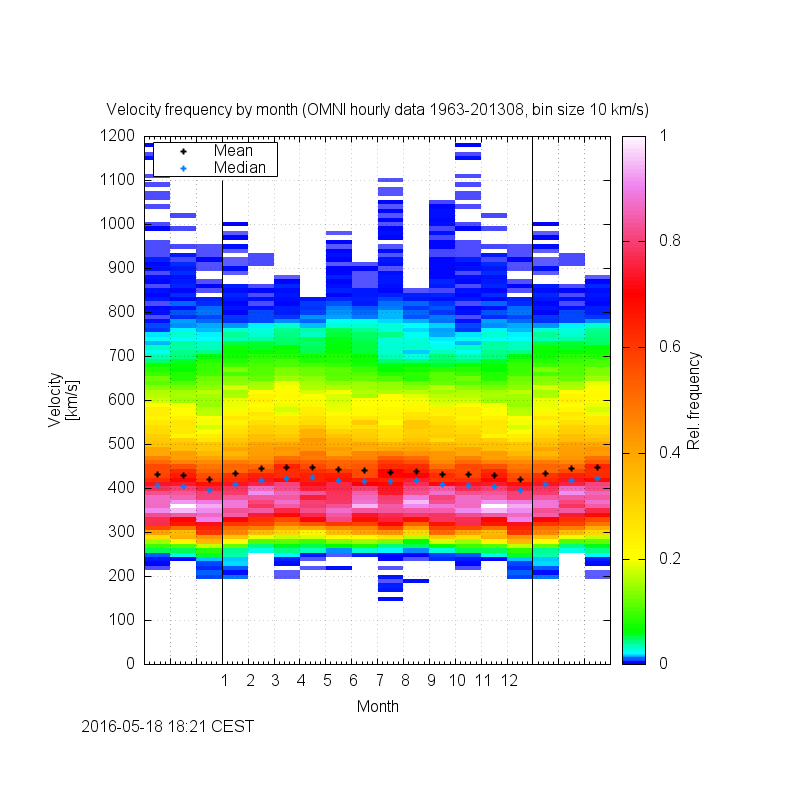
\includegraphics[width=0.3\textwidth]{figures_of_mine/gnuplots/OMNI_monthly_freq_V_gps.png}
	\caption{Diagram of the velocity frequency by month for the period 1963/01--2013/08. Mean and median values are shown as well.}
	\label{fig:OMNI_monthly_freq_V_gps}
\end{figure}
\begin{figure}[htb]
	\centering
	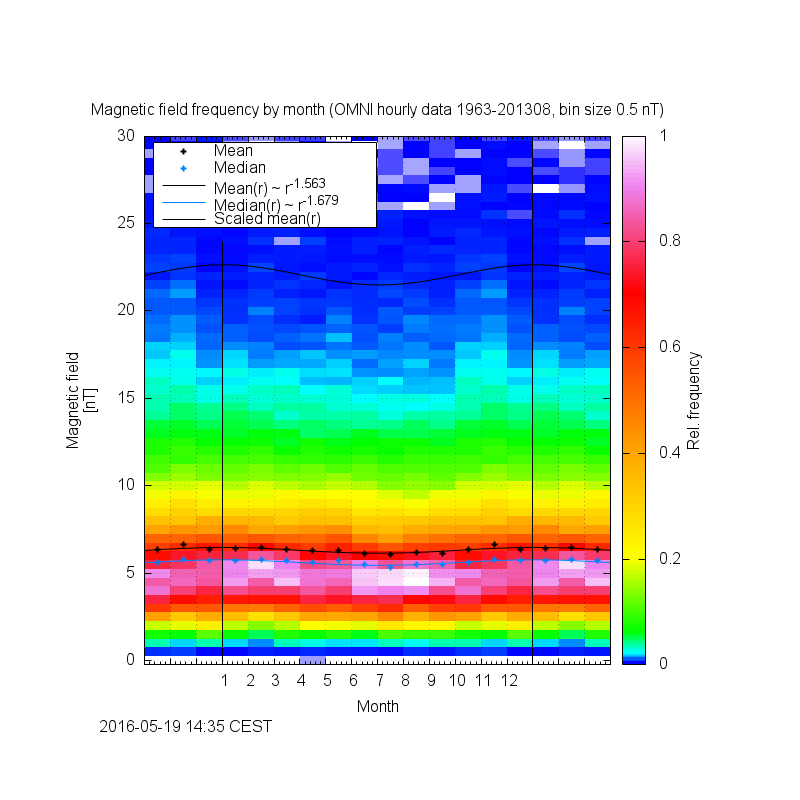
\includegraphics[width=0.3\textwidth]{figures_of_mine/gnuplots/OMNI_monthly_freq_B_a_gps.png}
	\caption{Diagram of magnetic field frequency by month for the period 1963/01--2013/08. Mean and median values are shown as well as the expected course from the solar distance variation (obtained from Helios data).}
	\label{fig:OMNI_monthly_freq_B_a_gps}
\end{figure}
make 4-panel figure...\\

derived exponent values from simple trigonometric fit on monthly values:\\
$c_n = -2.234$\\
maybe figure?\\

expected influence from Earth's perihelion/aphelion (see Appendix...) distance vs observations\\
we expect for the mean proton density (scaling law $n(r) \propto r^{-2.114}$):\\
$n(0.983~au) = 7.098~cm^{-3}$\\
$n(1~au) = 6.845~cm^{-3}$\\
$n(1.017~au) = 6.605~cm^{-3}$\\
we expect for the magnetic field strength (paper scaling law $n(r) \propto r^{-1.662}$):\\
$B(0.983~au) = 5.870~nT$\\
$B(1~au) = 5.705~nT$\\
$B(1.017~au) = 5.547~nT$\\

% % % former outlook
Seasonal effects from the orbit of the Earth have an influence on the OMNI data set, as it represents measurements located at the bow shock of the magnetosphere. These effects include the Earth's solar distance and its heliographic latitude. It would be valuable to estimate how large the resulting errors for the models are.

\subsection{Latitude dependency}
refer to Ulysses \autoref{fig:McComas2008_Ulysses_orbit}\\
Ulysses swoops polar plots...\\

see Schwenn1990's~Fig.~3.14\\
see also \citet{Schwenn1990} p.~127\\
see also \citet{Richardson1995}\\
Balogh et al. (1999) p. 162 ff (origin and formation of CIRs in inner heliosphere with Helios data; latitude V dependence)\\

Helios latitude; see \autoref{fig:latitude_frequency_4_thesis_plot}
\begin{figure}[htb]
	\centering
	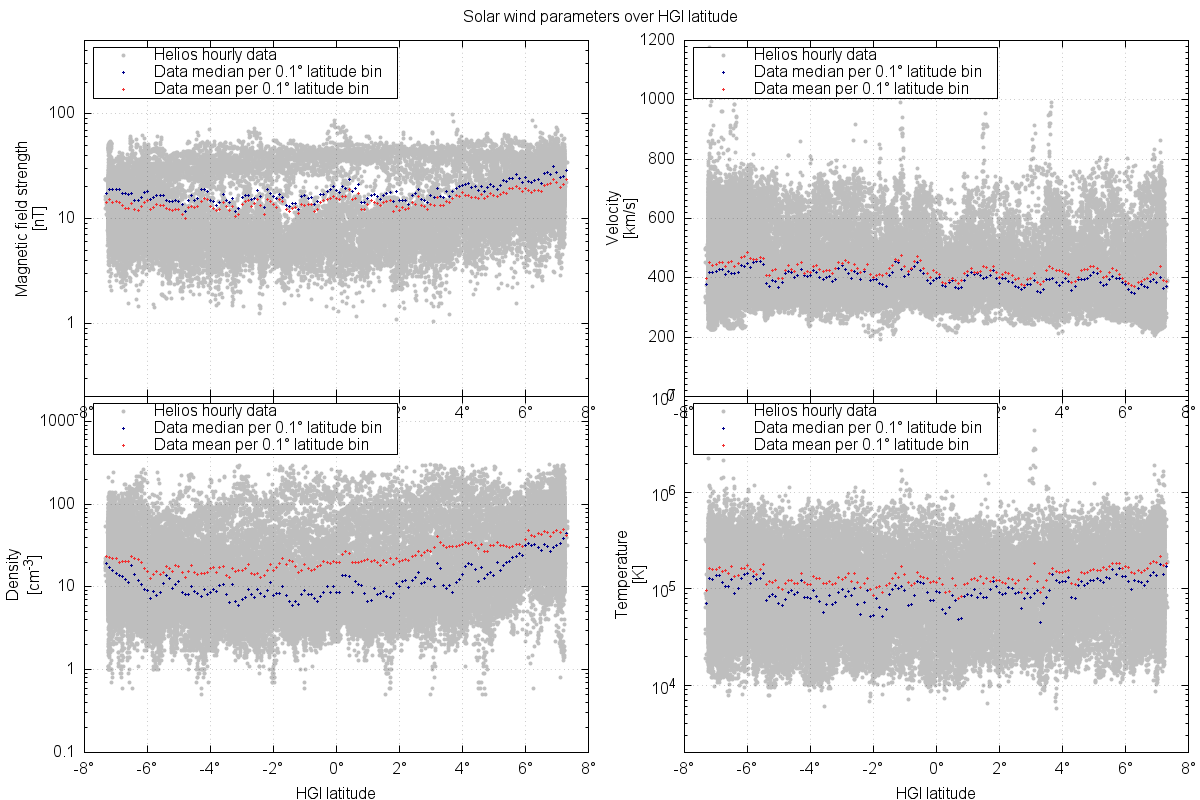
\includegraphics[width=0.5\textwidth]{figures_of_mine/gnuplots/latitude_frequency_4_thesis_plot.png}
	\caption{The four solar wind parameter's HGI latitude dependency. Their mean and median values per \SI{0.1}{\degree} bin are plotted as well. I added a random distance value of up to \SI{+-0.005}{\au} in order to make the distribution visible in this plot.}
	\label{fig:latitude_frequency_4_thesis_plot}
\end{figure}

with the exponential dependencies to 1~au projected solar wind parameters; there are only small changes with latitude in the range \SIrange{-7.25}{7.25}{\degree}\\
have a look on distribution widths...\\

dependence from latitude in interval \SIrange{-7.25}{7.25}{\degree} in Helios data negligible?, see \autoref{fig:latitude_frequency_rcorrected_v3_4_thesis_plot}.\\
\begin{figure}[htb]
	\centering
	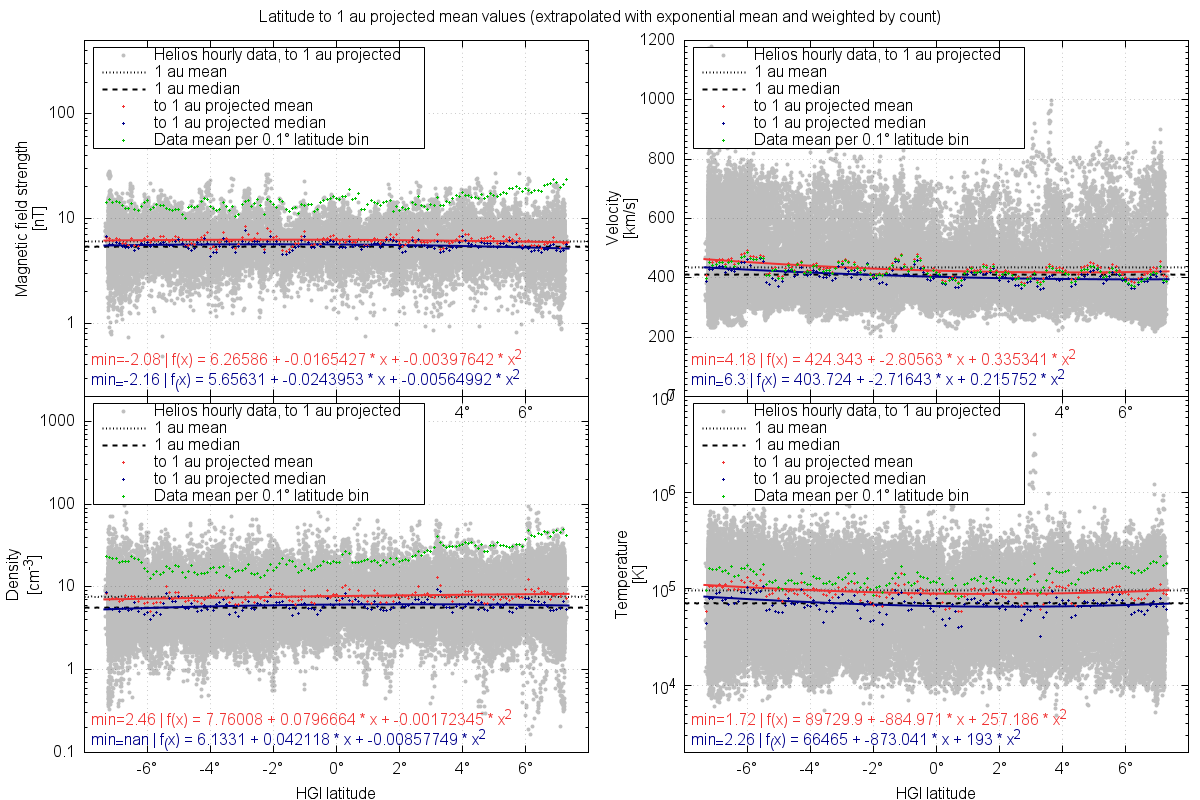
\includegraphics[width=0.5\textwidth]{figures_of_mine/gnuplots/latitude_frequency_rcorrected_v3_4_thesis_plot.png}
	\caption{Solar wind parameters projected to 1~au with respect to latitude. And their mean values, including weighted fit. I added a random distance value of up to \SI{+-0.005}{\au} in order to make the distribution visible in this plot. add projected median...}
	\label{fig:latitude_frequency_rcorrected_v3_4_thesis_plot}
\end{figure}
estimate error ranges from latitude influence...\\

...plot Ulysses data into plot?\\

%latitude variation negligible?
influence from latitude variation in data negligible? (see Ulysses \autoref{fig:McComas2008_Ulysses_orbit} in introduction). Helios probes within ecliptic => variation span equal to solar tilt: \SIrange{-7.25}{7.25}{\degree}\\
big part of Helios data is from latitudes $>\pm5$°, see Figure~XX (data count over latitude) and see \autoref{fig:Helios12_orbits_ecliptic_polar} (Helios orbit polar plane in data section)\\

The Helios magnetic field and plasma data frequency over heliocentric distance and over heliographic latitude are plotted in \autoref{fig:helios_data_frequency}.\\
\begin{figure}[htb]
	\centering
	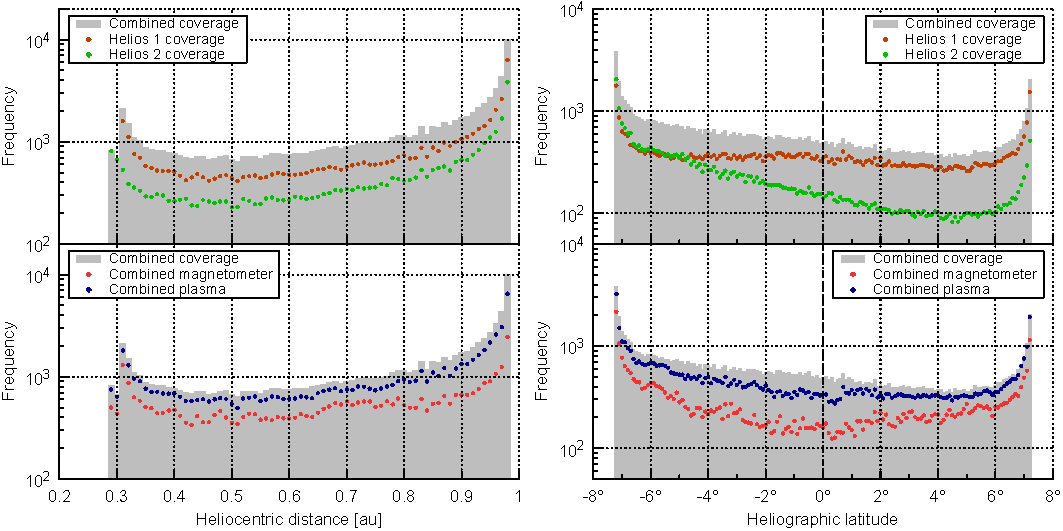
\includegraphics[width=0.5\textwidth]{figures_of_mine/gnuplots/helios_data_frequency.pdf}
	\caption[\lofimage{figures_of_mine/gnuplots/helios_data_frequency.pdf}]
	{Helios data frequency over heliocentric distance with bins of \SI{0.01}{au} (left panels) and over heliographic latitude with bins of \SI{0.1}{\degree} (right panels). The frequency data is based on the hourly merged magnetometer and plasma data sets for Helios~1 and Helios~2. The top panels show the frequencies for Helios~1 and Helios~2 individually and the bottom panels those for the magnetometer and plasma data.}
	\label{fig:helios_data_frequency}
\end{figure}

\subsection{Radial evolution of solar wind structures}
Helios event lists HSSs, SLOWs, CIRs, CMEs...; event lists for all Helios data\\
see Liu2004 for Helios ICME list and radial dependencies of $B$, $n$, $T$ and $v$...\\

\SI{200}{\km\per\s} slow solar wind at \SI{10}{\Rs} is in agreement with blob measurements from Wang2000\\

very slow sw (VSSW) gets accelerated; see Sanchez-Diaz2016:\\
%"The reported in situ measurements suggest that the properties of VSSW are a continuation of the slow wind toward lower speeds: higher densities, higher proton fluxes, and lower temperatures, thereby extending well-known scaling laws [Lopez and Freeman, 1986; Hundhausen et al., 1970] down to speeds as low as 200 km/s."\\
%"The VSSW has a number of interesting properties that suggest it may be the interplanetary signature of long HPS crossings."\\

radial diameter of MCs increase between 0.3~au and 4.3~au proportional to the distance as $r^{0.8}$ \citep{Bothmer1998}\\
MC central axial magnetic field strength radial density dependence $B = 18.1\,r^{-1.64}$ \citet{Leitner2007}\\
MC average diameter $D = 0.23\,r^{1.14}$ \citet{Leitner2007}

sw structure marked plots\\


